\section{Thiết kế giao diện người dùng (UI)}
Phần này trình bày hình ảnh giao diện thực tế của hệ thống LumiCinema kèm theo \textbf{Danh sách thành phần} và \textbf{Danh sách biến cố} tương ứng cho từng màn hình chính.

% --- 1. Trang chủ ---
\subsection{Màn hình Trang chủ}
\begin{figure}[H]
  \centering
  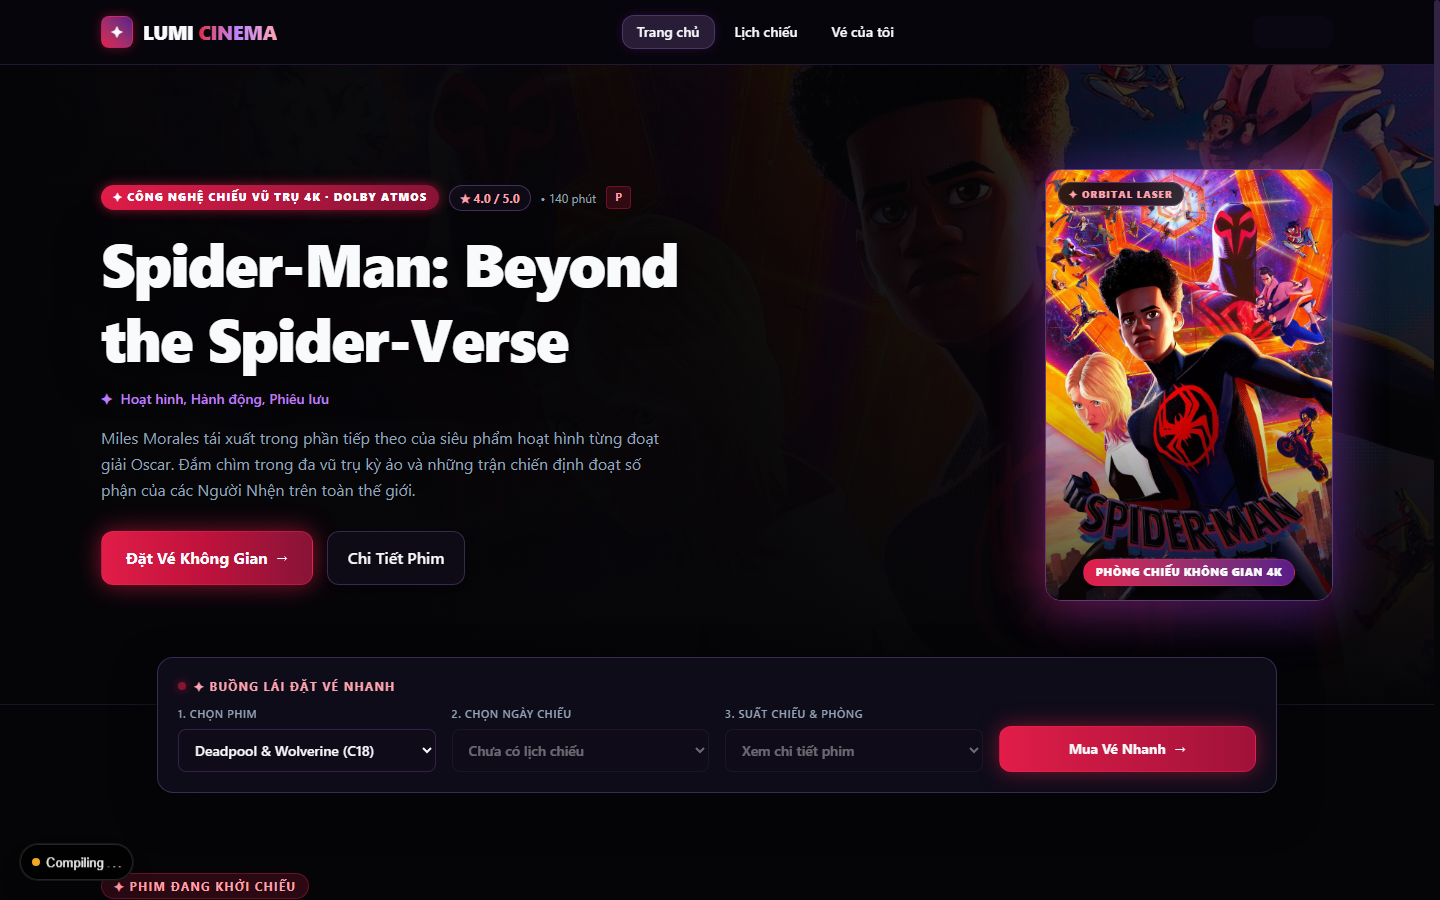
\includegraphics[width=\textwidth,height=0.55\textheight,keepaspectratio]{images/ui/ui_01_trang_chu.png}
  \caption{Giao diện Trang chủ LumiCinema}
  \label{fig:ui_01}
\end{figure}
\begin{itemize}[leftmargin=1.2cm]
  \item \textbf{Danh sách thành phần:} Thanh điều hướng (Logo, Phim, Vé của tôi, Đăng nhập/Đăng ký), Banner phim nổi bật, Thanh tìm kiếm \& lọc thể loại/trạng thái phim, Lưới thẻ phim (Poster, tên phim, thời lượng, đánh giá sao, nút Đặt vé).
  \item \textbf{Danh sách biến cố:} Nhấn chọn phim $\rightarrow$ chuyển trang Chi tiết phim; Nhập từ khóa/chọn bộ lọc $\rightarrow$ lọc danh sách phim theo thời gian thực; Nhấn Đăng nhập/Đăng ký $\rightarrow$ mở trang xác thực.
\end{itemize}

% --- 2. Đăng nhập ---
\subsection{Màn hình Đăng nhập}
\begin{figure}[H]
  \centering
  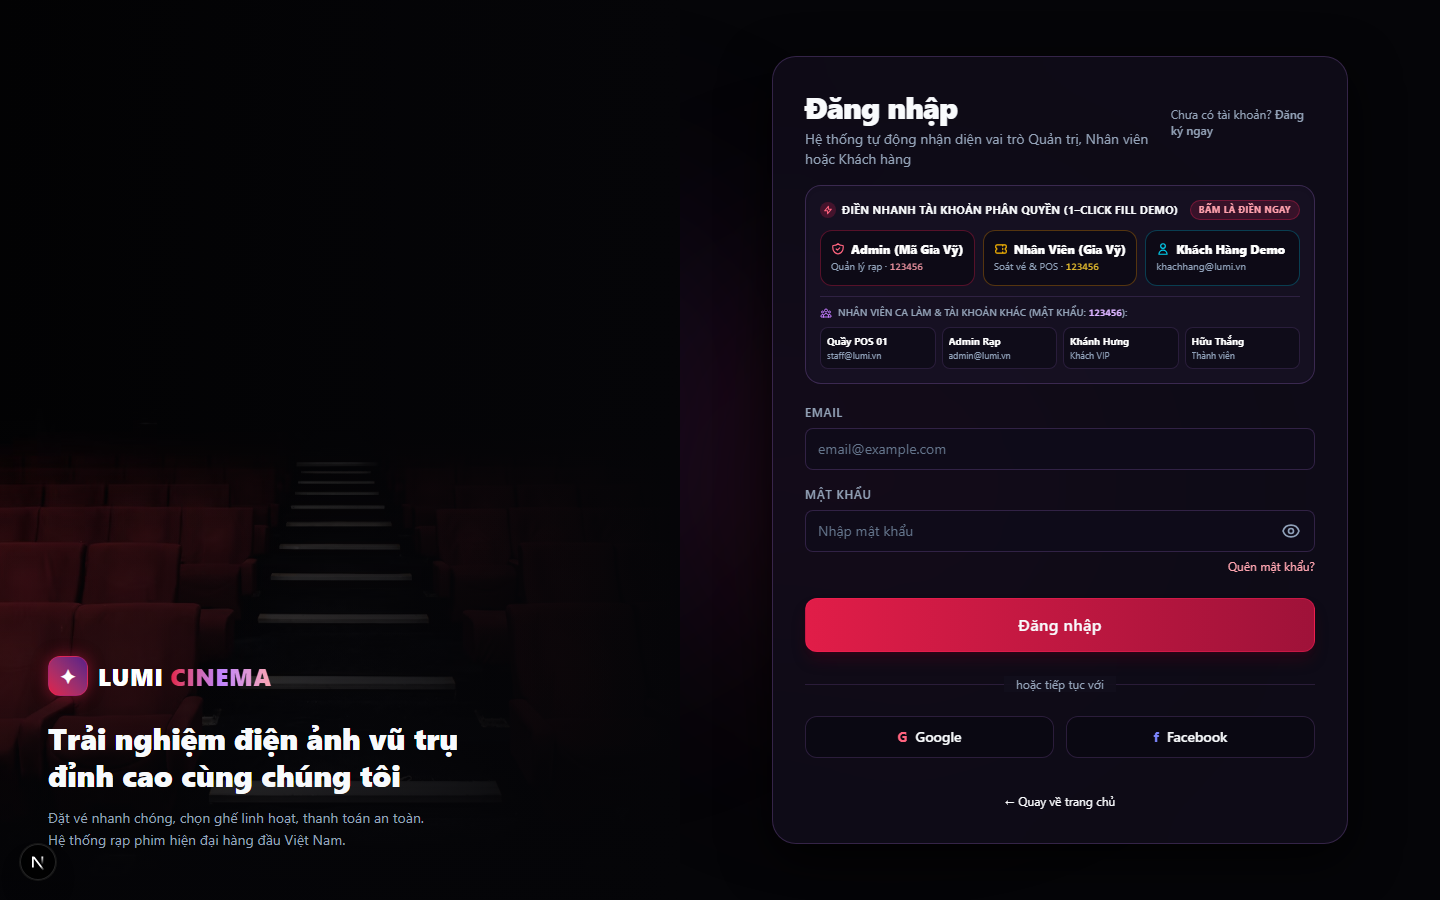
\includegraphics[width=\textwidth,height=0.55\textheight,keepaspectratio]{images/ui/ui_02_dang_nhap.png}
  \caption{Giao diện Đăng nhập}
  \label{fig:ui_02}
\end{figure}
\begin{itemize}[leftmargin=1.2cm]
  \item \textbf{Danh sách thành phần:} Ô nhập Email, Ô nhập Mật khẩu, Nút Đăng nhập, Liên kết chuyển sang trang Đăng ký, Vùng hiển thị thông báo lỗi.
  \item \textbf{Danh sách biến cố:} Nhấn ``Đăng nhập'' $\rightarrow$ gọi \texttt{POST /api/auth/login}, xác thực mật khẩu, lưu phiên làm việc (JWT Cookie) và điều hướng theo vai trò (Khách hàng / Nhân viên / Admin).
\end{itemize}

% --- 3. Đăng ký ---
\subsection{Màn hình Đăng ký tài khoản}
\begin{figure}[H]
  \centering
  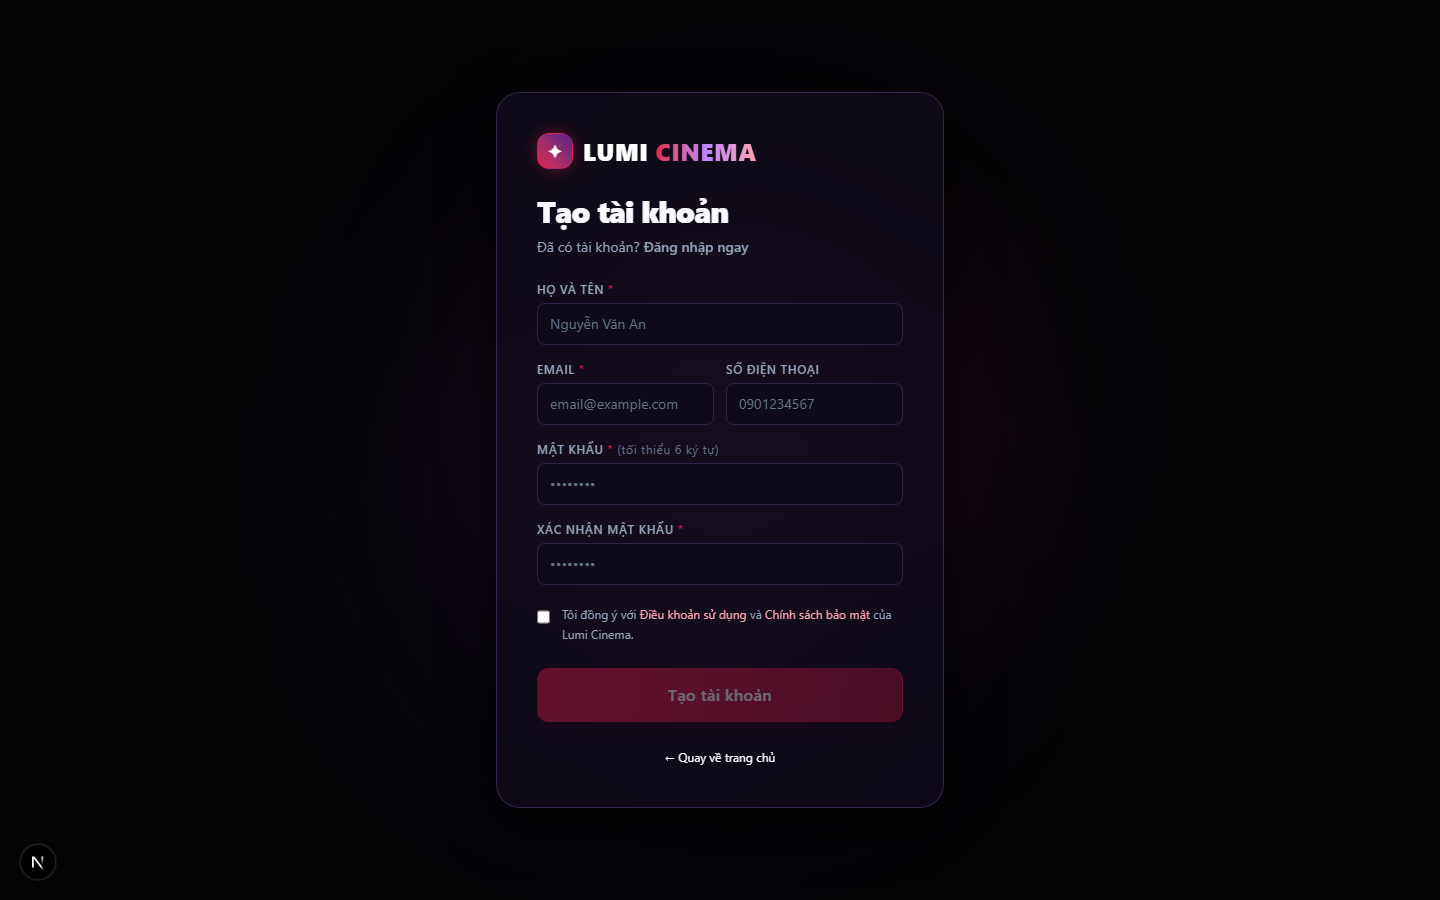
\includegraphics[width=\textwidth,height=0.55\textheight,keepaspectratio]{images/ui/ui_03_dang_ky.png}
  \caption{Giao diện Đăng ký tài khoản}
  \label{fig:ui_03}
\end{figure}
\begin{itemize}[leftmargin=1.2cm]
  \item \textbf{Danh sách thành phần:} Ô nhập Họ tên, Email, Số điện thoại, Mật khẩu, Xác nhận mật khẩu, Nút Đăng ký.
  \item \textbf{Danh sách biến cố:} Nhấn ``Đăng ký'' $\rightarrow$ kiểm tra hợp lệ dữ liệu, gọi \texttt{POST /api/auth/register}, mã hóa mật khẩu bằng bcrypt và tạo tài khoản khách hàng mới.
\end{itemize}

% --- 4. Chi tiết phim ---
\subsection{Màn hình Chi tiết phim và Chọn suất chiếu}
\begin{figure}[H]
  \centering
  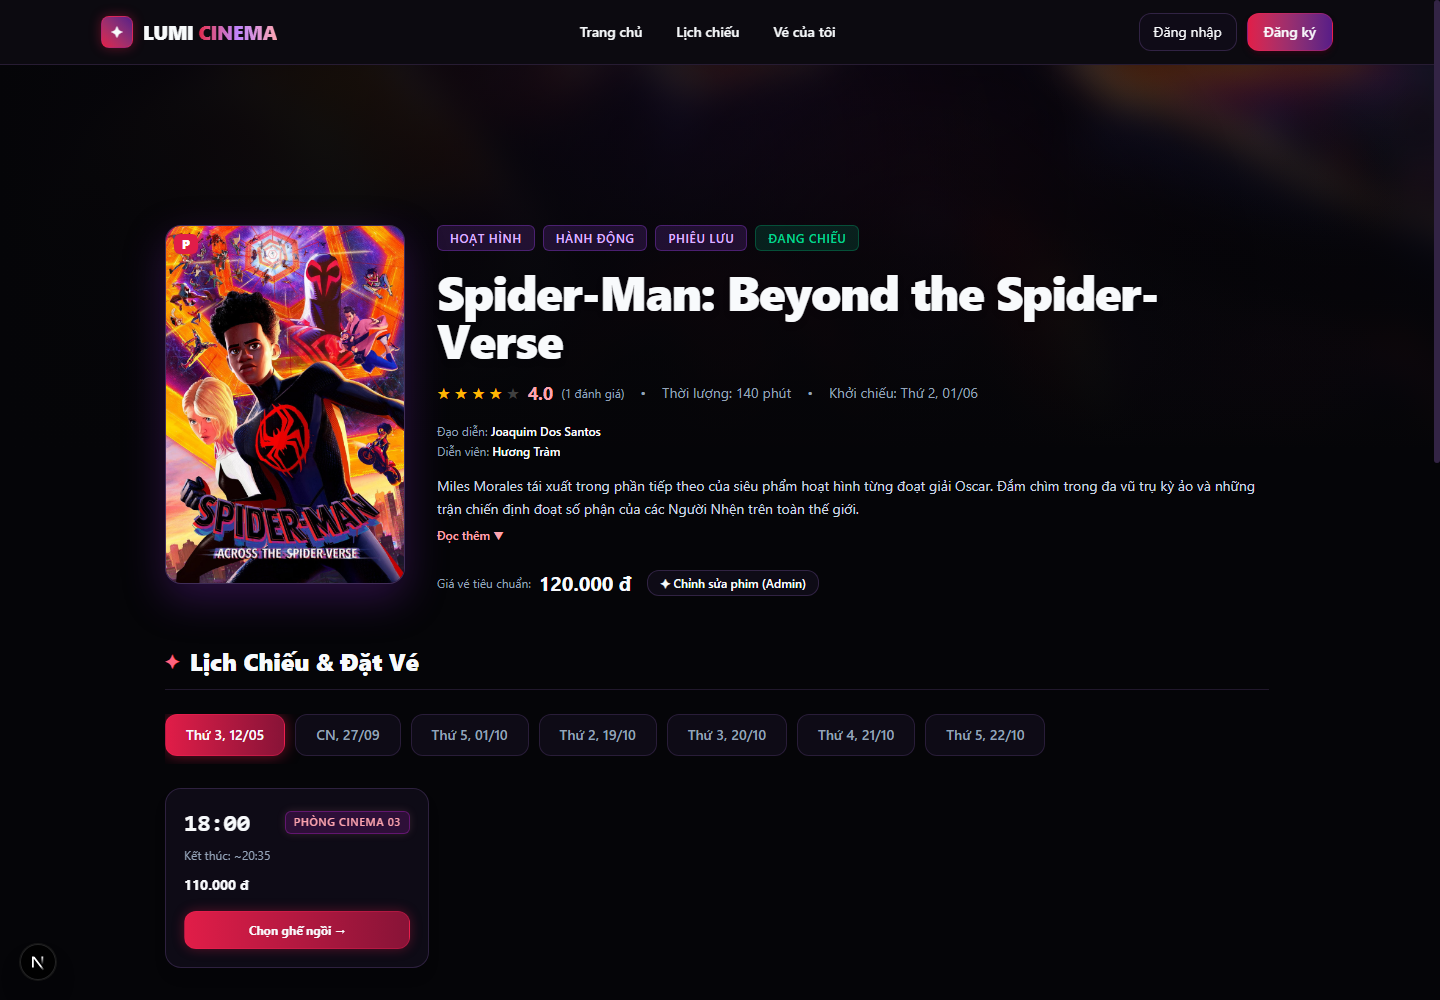
\includegraphics[width=\textwidth,height=0.55\textheight,keepaspectratio]{images/ui/ui_04_chi_tiet_phim.png}
  \caption{Giao diện Chi tiết phim và Suất chiếu}
  \label{fig:ui_04}
\end{figure}
\begin{itemize}[leftmargin=1.2cm]
  \item \textbf{Danh sách thành phần:} Poster, Thông tin phim (thể loại, thời lượng, mô tả, điểm đánh giá trung bình), Bộ chọn ngày chiếu, Danh sách nút khung giờ suất chiếu, Khu vực đánh giá phim (1--5 sao và bình luận).
  \item \textbf{Danh sách biến cố:} Chọn ngày chiếu $\rightarrow$ cập nhật danh sách suất chiếu; Nhấn khung giờ $\rightarrow$ chuyển sang màn hình Chọn ghế; Gửi đánh giá $\rightarrow$ gọi \texttt{POST /api/reviews}.
\end{itemize}

% --- 5. Chọn ghế ---
\subsection{Màn hình Chọn ghế (Sơ đồ 50 ghế A1--E10)}
\begin{figure}[H]
  \centering
  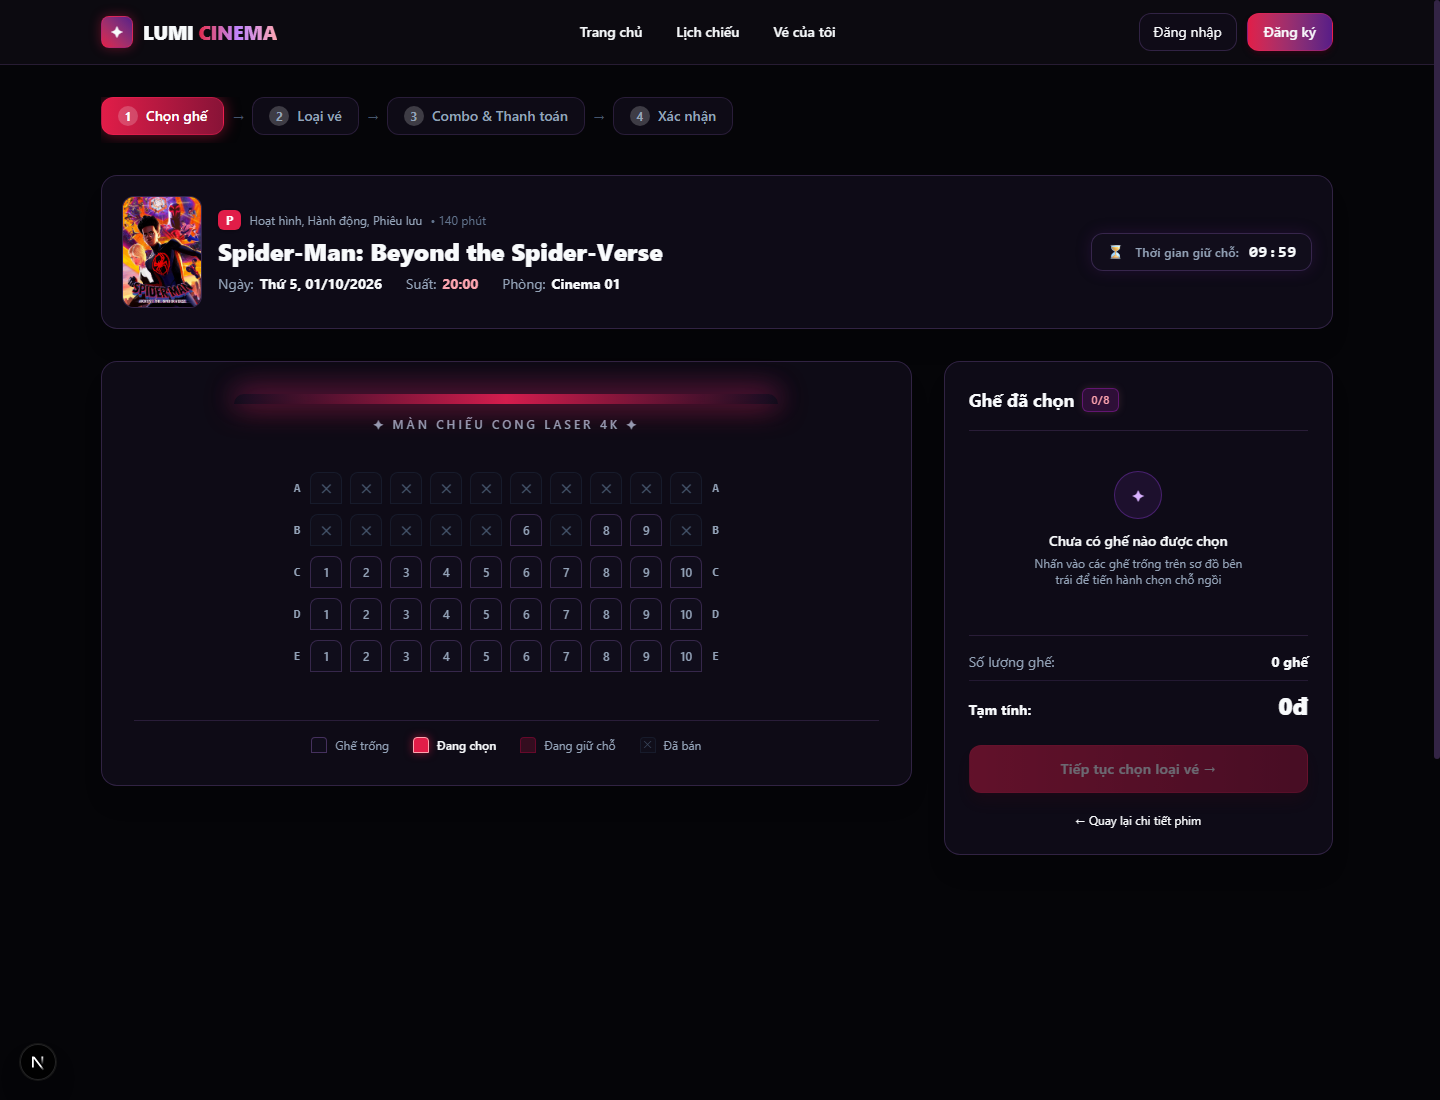
\includegraphics[width=\textwidth,height=0.55\textheight,keepaspectratio]{images/ui/ui_05_chon_ghe.png}
  \caption{Giao diện Chọn ghế phòng chiếu (5 hàng A--E, 10 cột 1--10)}
  \label{fig:ui_05}
\end{figure}
\begin{itemize}[leftmargin=1.2cm]
  \item \textbf{Danh sách thành phần:} Thanh màn hình chiếu, Lưới 50 nút ghế (phân màu Trống / Đang chọn / Đang giữ / Đã đặt), Bộ chọn loại vé (Người lớn / Sinh viên / Trẻ em), Bảng tóm tắt ghế đã chọn \& tạm tính, Nút Tiếp tục.
  \item \textbf{Danh sách biến cố:} Nhấn chọn/bỏ chọn ghế $\rightarrow$ cập nhật danh sách ghế và tổng tiền; Nhấn ``Tiếp tục'' $\rightarrow$ giữ ghế tạm thời (TTL) và chuyển sang bước Chọn Combo.
\end{itemize}

% --- 6. Chọn Combo & Thanh toán ---
\subsection{Màn hình Chọn Combo, Áp dụng Voucher và Thanh toán}
\begin{figure}[H]
  \centering
  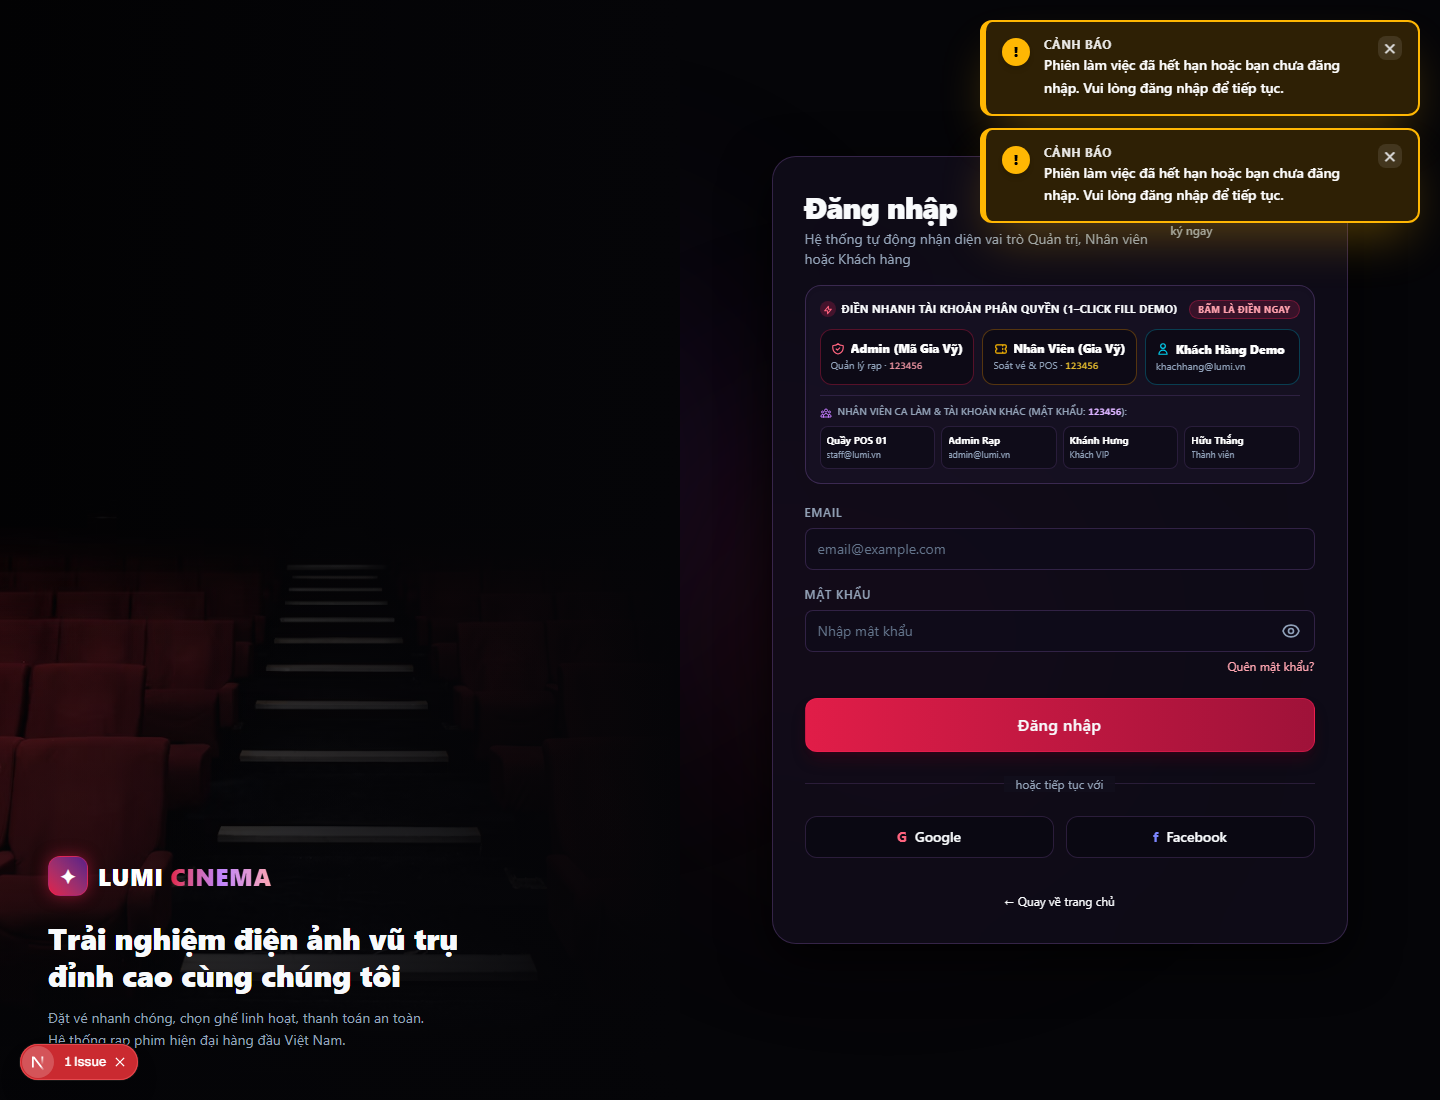
\includegraphics[width=\textwidth,height=0.55\textheight,keepaspectratio]{images/ui/ui_06_chon_combo.png}
  \caption{Giao diện Chọn Combo bắp nước và Thanh toán}
  \label{fig:ui_06}
\end{figure}
\begin{itemize}[leftmargin=1.2cm]
  \item \textbf{Danh sách thành phần:} Danh sách thẻ Combo (hình ảnh, giá, tồn kho, nút tăng/giảm số lượng), Ô nhập mã Voucher \& nút Áp dụng, Bộ chọn cổng thanh toán (ZaloPay / VNPay Gateway), Bảng tổng kết thanh toán, Nút Thanh toán.
  \item \textbf{Danh sách biến cố:} Tăng/giảm combo $\rightarrow$ cập nhật tổng tiền theo tồn kho; Áp dụng voucher $\rightarrow$ kiểm tra hợp lệ \& trừ giảm giá; Nhấn Thanh toán $\rightarrow$ tạo đơn và chuyển hướng sang cổng ZaloPay/VNPay (\texttt{/payments/zalopay-mock} hoặc \texttt{/payments/vnpay-mock}) để xác nhận trừ số dư.
\end{itemize}

% --- 7. Nhân viên POS ---
\subsection{Màn hình Nhân viên quầy (Bán vé, Soát vé \& Hủy vé sự cố)}
\begin{figure}[H]
  \centering
  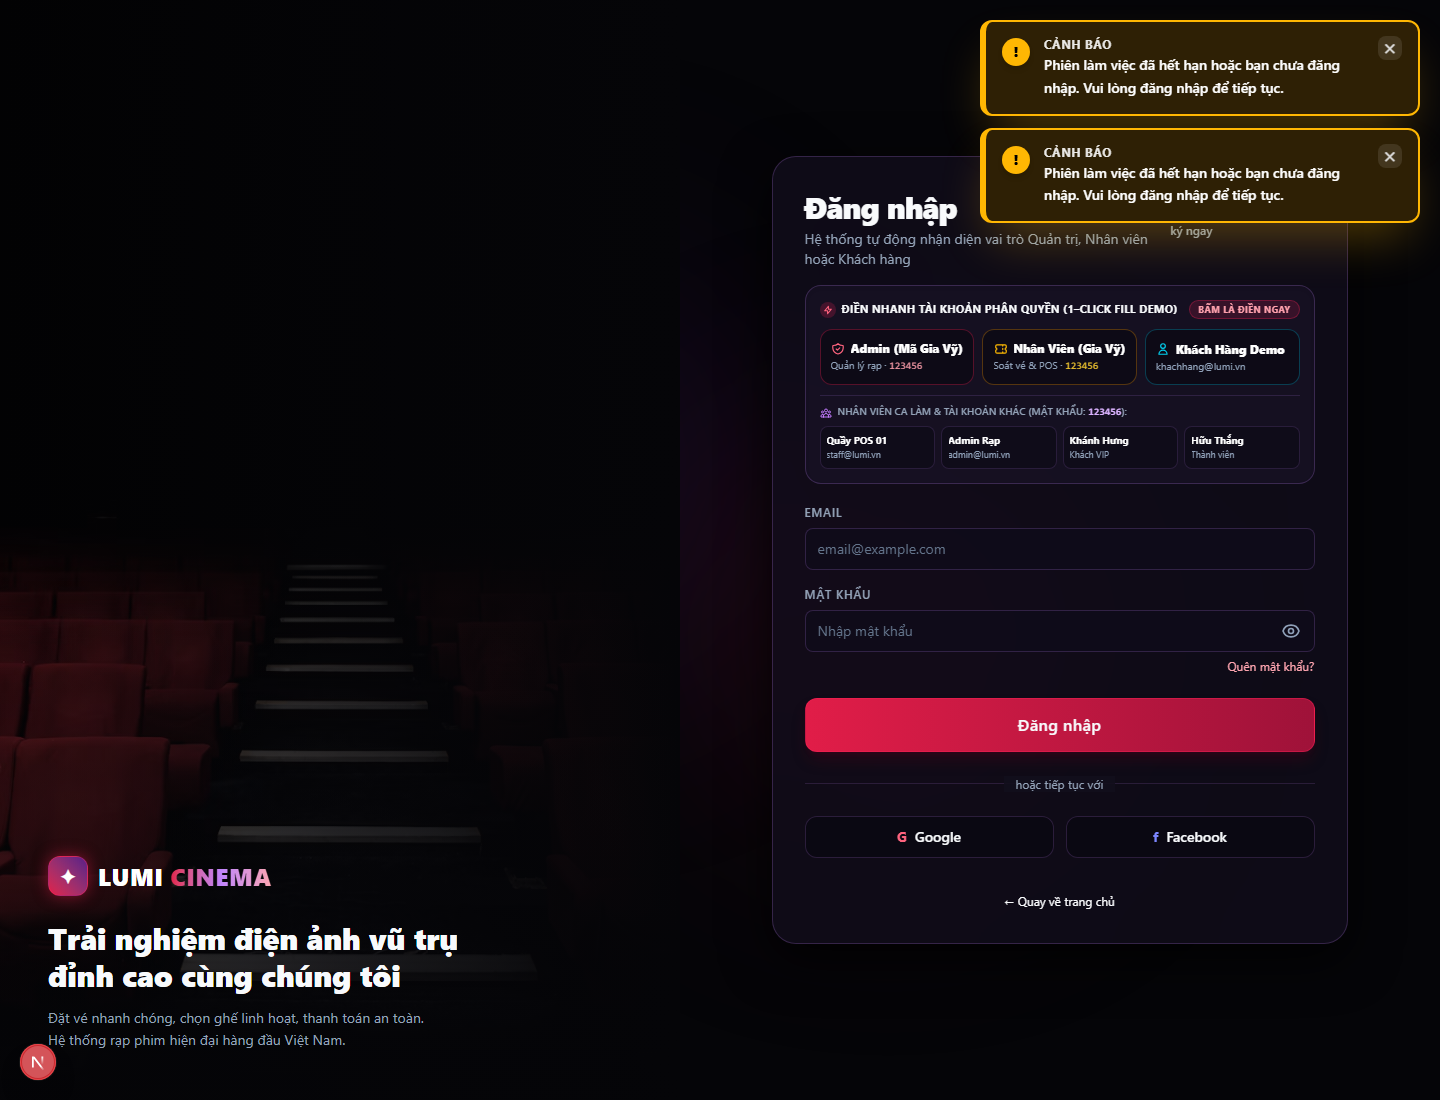
\includegraphics[width=\textwidth,height=0.55\textheight,keepaspectratio]{images/ui/ui_08_nhan_vien_staff.png}
  \caption{Giao diện làm việc của Nhân viên quầy (POS)}
  \label{fig:ui_08}
\end{figure}
\begin{itemize}[leftmargin=1.2cm]
  \item \textbf{Danh sách thành phần:} Các tab nghiệp vụ (Bán vé tại quầy, Soát vé \& Giao combo, Tra cứu \& Hủy vé), Ô tìm kiếm mã vé/SĐT, Sơ đồ ghế POS, Modal xử lý hủy vé sự cố 1 bước (chọn Hoàn 100\% tiền mặt hoặc Cấp voucher 100\%).
  \item \textbf{Danh sách biến cố:} Xác nhận bán vé $\rightarrow$ thu tiền, xuất vé; Quét/nhập mã vé $\rightarrow$ xác nhận vào rạp hoặc giao combo; Xác nhận ép hủy sự cố $\rightarrow$ giải phóng ghế, lưu log, lập chứng từ hoàn tiền/voucher và gửi email tự động.
\end{itemize}

% --- 8. Admin Dashboard ---
\subsection{Màn hình Quản trị và Báo cáo doanh thu (Admin Dashboard)}
\begin{figure}[H]
  \centering
  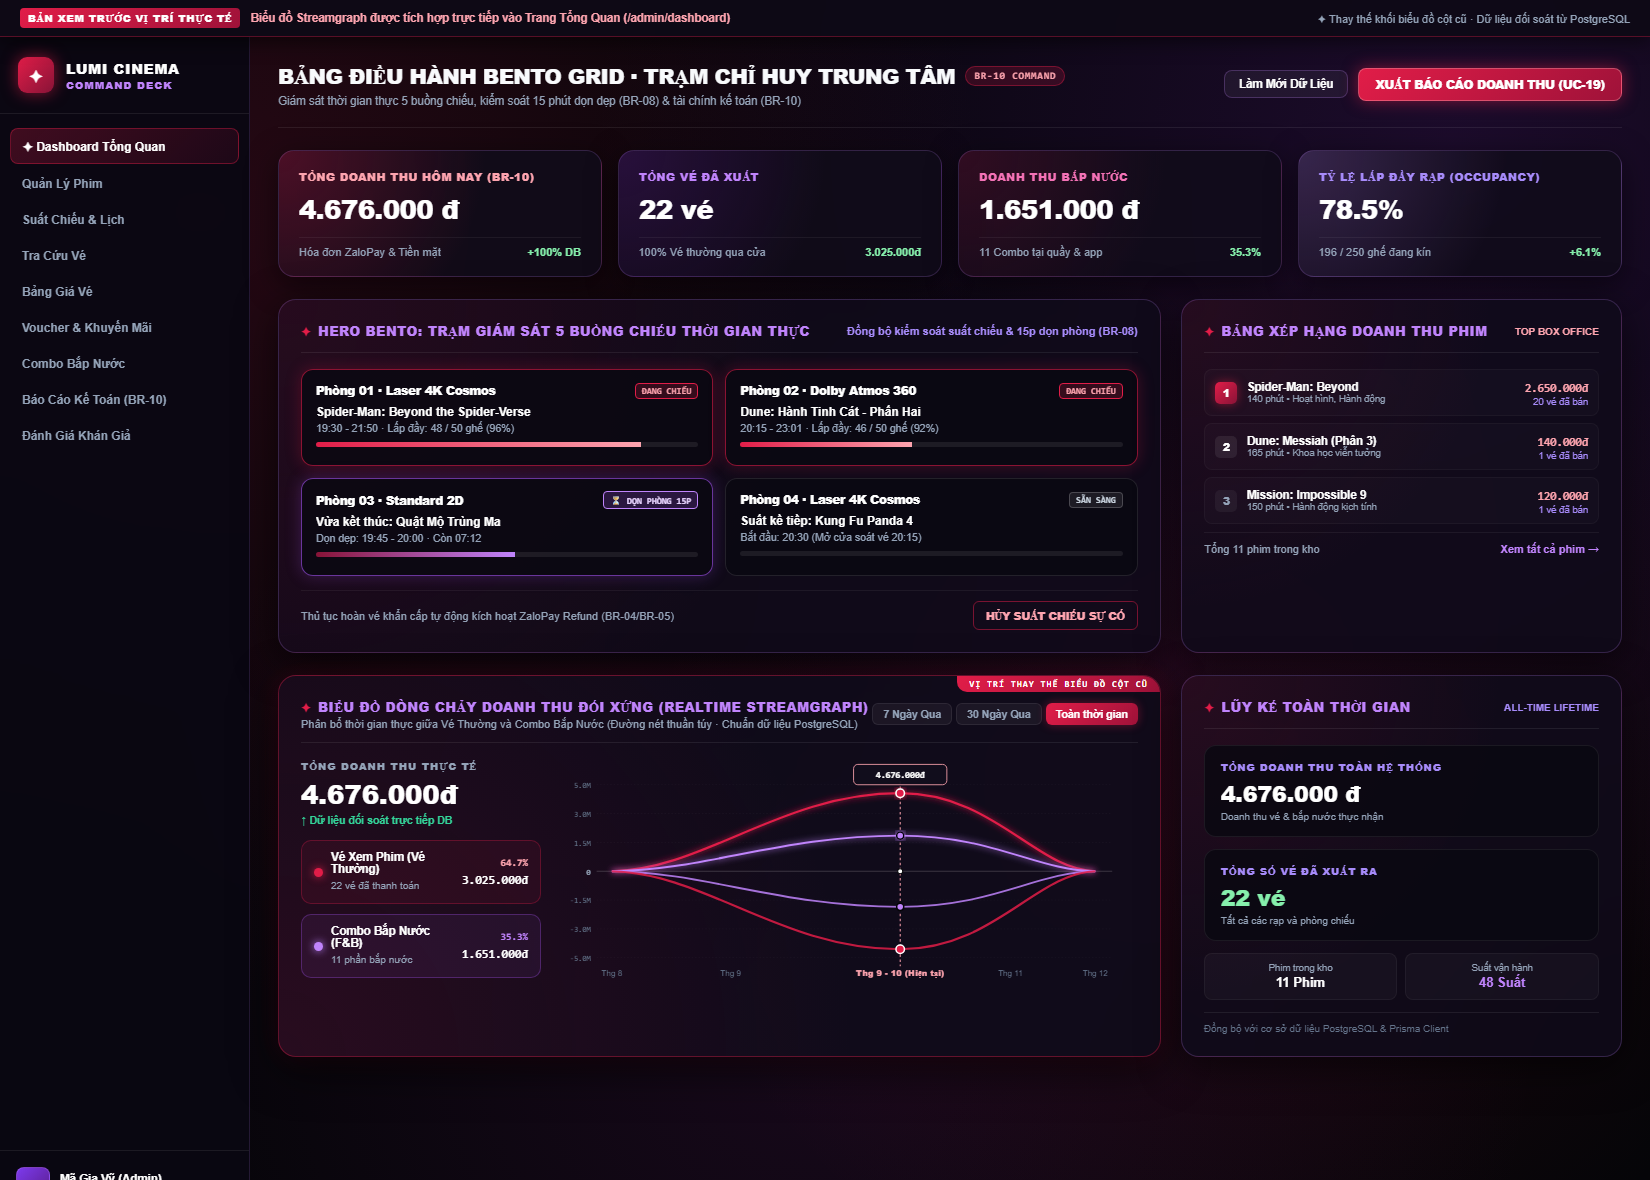
\includegraphics[width=\textwidth,height=0.55\textheight,keepaspectratio]{images/ui/ui_09_admin_dashboard_streamgraph.png}
  \caption{Giao diện Admin Dashboard với biểu đồ Streamgraph doanh thu}
  \label{fig:ui_09}
\end{figure}
\begin{itemize}[leftmargin=1.2cm]
  \item \textbf{Danh sách thành phần:} Thanh điều hướng quản trị (Dashboard, Phim, Suất chiếu, Combo, Voucher), Thẻ KPI tổng quan (Tổng doanh thu, Vé đã bán, Tỷ lệ lấp đầy), Biểu đồ Streamgraph doanh thu theo thời gian, Bộ lọc thời gian/phim/suất chiếu, Nút Xuất báo cáo CSV.
  \item \textbf{Danh sách biến cố:} Thay đổi bộ lọc $\rightarrow$ truy vấn lại số liệu tổng hợp vé \& combo; Nhấn ``Xuất CSV'' $\rightarrow$ tải về tệp báo cáo doanh thu định dạng CSV.
\end{itemize}
